\documentclass{article}

  \title{Opening the third eye?  \\ Are Experiences with Psychedelics more Spiritual than non-psychedelics?}
  \author{Isobel Smith}
  \date{20/11/2016}
  
\usepackage{amsmath}
\usepackage{booktabs}
\usepackage{graphicx}
\usepackage{float}
\usepackage{listings}
\usepackage{color}
\usepackage{url}

\graphicspath{}

 \begin{document}
\maketitle

\section{Research Question}

Psychoactive, or psychadelic drugs, such as mushrooms and LSD, are believed by many users to enhance conciousness, giving practitioners a spiritual, or even religious, experience \cite{letcher} \cite{watts}. Entrenched in indigenous culture, the use and popularity of these drugs is growing globally, despite prohibition, \cite{letcher} \cite{rager}. According to Letcher, practitioners experiences' with these drugs are "weighted", meaning that many people encounter similar hallucinations whilst on these drugs.  According to my own research, psychadelic drugs are amongst the most popular recreational drugs across both genders (see figure 1). What is it about the experiences people have on these drugs that make them so popular? Do people have shared or similar experiences? Is there a common goal or experience that these drug users strive for?\\

In order to answer these questions I will datamine the Erowid experience vaults. This database is built on drug users documenting their own personal experiences, and therefore provides valuable insights into the popularity and the appeal of such substances. 


\section{context of research}
The growth in use and popularity of pyschedelic drugs makes it an increasingly important area of study, as such drugs can have wide social implications. The most prominant example of this would be during the 70's, after the popularism of LSD led to the development of a subculture, spawning its own music and language \cite{letcher}. The prohibition of psychedelic drugs helps to build the (the users? the popularism? the identity?) , as an underground culture has grown around these users. Those who do use psychedelic drugs become part of an exclusive club. which, due to the illegality of the substances, has its own language and customs, that only the indoctrinated can understand. \\


\section{Data collection}
The Erowid Experience vaults form the database for my research. The data is based on drug users documenting their own experiences, so offers a unique insight into the drug culture. \\ 
The webpage HTML was parsed using beautiful soup to filter and sort the drug experiences. 

The data (as of the time of writing) contained 24, 843 experiences. However, as these were split across several different substances, this led to (get amount) LSD experience reports, (number) Salvia reports, and (number) mushroom reports. Therefore, in order to strengthen the research (another potential sight) was used. 

\section{Methodology}

Each of the experiences were downloaded, and processed using beautiful soup. Initially a dict was created in the form of:

\begin{lstlisting}
{experience_id {drug: gender}}
\end{lstlisting}

The genders were seperated into male and female, and charts made to compare whether drug use differed across users:

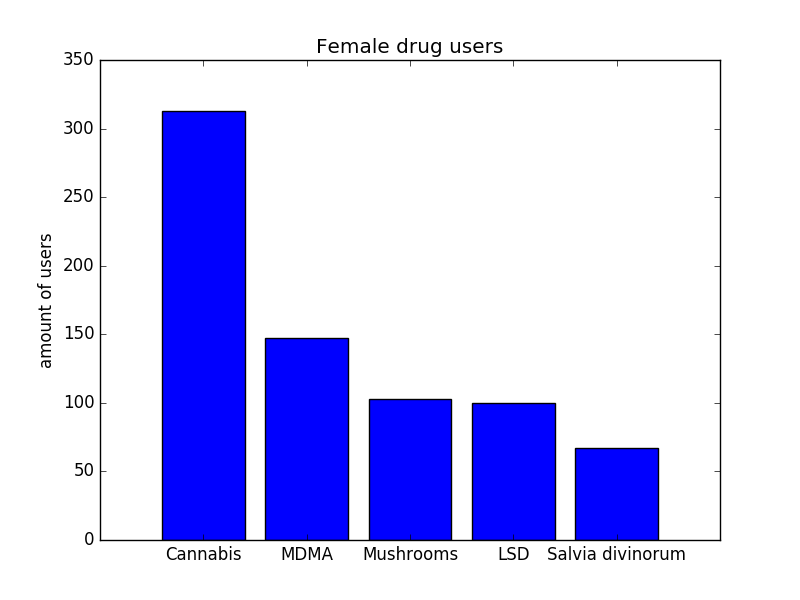
\includegraphics{graphs/top_female_drugs}

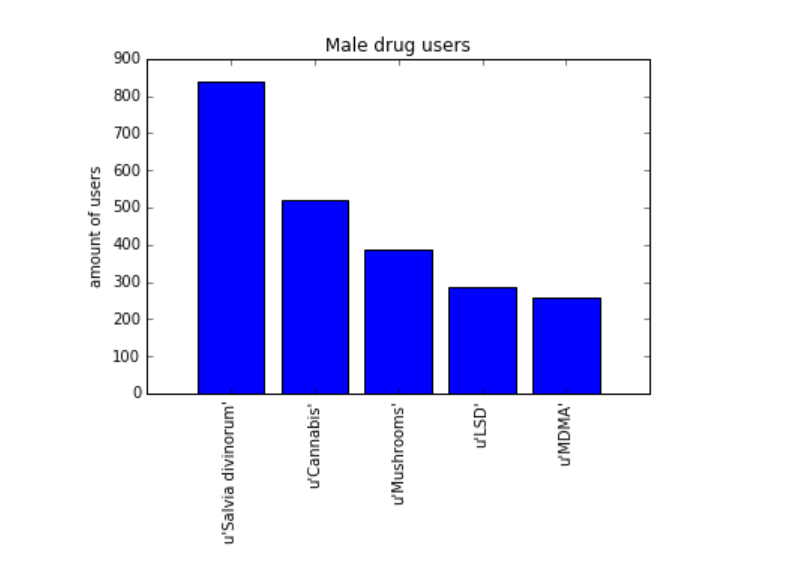
\includegraphics{graphs/top_male_drugs}

As you can see the differences are not substantial. Mushrooms and LSD are amongst the most popular drugs used, and therefore highlights the relevance of my research question. 

The next step was to find all the reports which related to Mushrooms and LSD, and a count of the most frequent words was made. The text was lowered and stopwords removed, however more text processing could be done here to improve results:

\begin{lstlisting}
print word_count(tokenised).most_common(30)

[('like', 115720), ('would', 85580), ('felt', 84980), ('could', 69560), ('one', 65020), ('time', 64560), ('back', 61120), ('around', 52980), ('trip', 47460), ('started', 47440), ('get', 46260), ('really', 44680), ('got', 42820), ('went', 40700), ('feel', 40300), ('looked', 39840), ('thought', 39520), ('still', 38980), ('me.', 38760), ('go', 38640), ('seemed', 38000), ('going', 36560), ('see', 35500), ('began', 35440), ('everything', 35360), ('feeling', 34460), ('much', 32760), ('first', 32560), ('decided', 32080), ('even', 32000)]
\end{lstlisting}

As you can see the majority of the 30 most common words can be discarded, and if there is time, more work will be done to improve this. 

Finally, a (initially small) selection of words associated with spiritualism (as taken from wikipedia) and there subsequent word frequencies were found, and graphed:

\begin{lstlisting}
spiritual_words = ['god', 'spirit', 'heaven', 'hell', 'universe','magic','atheist', 'creation', 'concious', 'exist']
\end{lstlisting}

\includegraphics{graphs/pschedelic_spiritual_words}

The drugs were then split into a list of drugs classed as Serotonergic psychedelics and those that were not. This was done according to a list on \cite{wiki}

According to \cite{Lancaster}, word frequency is often normalised by Frequency per million words = ( frequency ÷ text no. words ) x 1,000,000 

Therefore the count of each of the spirit words (as defined above) were found for the pschedelic drugs and the non psychedelic drugs, and normalised. 

\begin{lstlisting}
spiritual words and normalised frequency psychedelics
{'heaven': 410.69744298138124, 'magic': 1174.9066090353438, 'universe': 2570.0153733039233, 'concious': 70.55381027709082, 'atheist': 54.586369003854465, 'creation': 275.15986008065414, 'exist': 805.0561088459625, 'god': 3301.9183209678495, 'hell': 3276.667483605522, 'spirit': 1329.7536558013799}
spiritual words and normalised frequency, rest of drugs
{'heaven': 190.43153902649394, 'magic': 548.4651050909255, 'universe': 1178.782362921309, 'concious': 32.85222456889807, 'atheist': 25.056781450854462, 'creation': 126.3975419854214, 'exist': 373.6244523005188, 'god': 1539.600015813613, 'hell': 1522.8954948463768, 'spirit': 610.2718326696998}
\end{lstlisting}

As we can see from the initial output, spiritual words do occur with more frequency in relation to psychedelics.

\subsection{Chi Square test}

A chi square test was carried out to compare whether spiritual words are over-represented in the psychoactive drugs as compared to the rest of the data. 

This was carries out using the normilised data:

\begin{lstlisting}
scipy.stats.chisquare(normalised_frequency,
                              f_exp=rest_normalised_frequency)
\end{lstlisting}
with the output:

\begin{lstlisting}
Power_divergenceResult(statistic=1296.8442867656056,
                                    pvalue=1.4860939588891628e-273)
\end{lstlisting}

The standard α value is 0.5, and therefore with a p-value of 1.49 we can accept the hypothesis, that spiritual words do occur more frequently in reports abuot psychedelics. Perhaps spiritualy curious people are drawn to psychedelics, or the hallucinagenic nature of the drugs causes users to question the nature of percieved reality. 

\section{Conclusion}

The initial text processing needs to be refined in order to improve results. However the word frequencies suggest that evidence can be found to suggest that there is spiritualism within the modern use of psychoactive drugs.

The project can be improved/ expanded upon by adding further drug experience webites, and looking at further spiritual words. The list of psychedelic drugs on wikipedia may not be comprehensive, and people may experience hallucinations on drugs other than the psychadelics. 

There are also problems with the data, for example, misspelled words may be missed from the search. 



\bibliographystyle{unsrt}
\bibliography{erowid-paper}

\end{document}